\documentclass[a4paper,10pt]{article}
\usepackage[english]{babel}
\usepackage[utf8]{inputenc}
\usepackage[toc,page]{appendix}
\usepackage{graphicx}
\usepackage{multirow}
\usepackage{array}

%Includes "References" in the table of contents
\usepackage[nottoc]{tocbibind}
\usepackage{titling}
\usepackage{setspace}




\parskip .8ex

%\setlength{\droptitle}{-10em}
\setlength{\topmargin}{-0.5in} % was -1

\usepackage{fancyheadings}
\usepackage{ifthen}
\usepackage{titlesec}
\setlength{\textheight}{9.7in} %was 10.2

%Begining of the document
\begin{document}

\title{\textbf{CSCM77: Computer Vision and Deep Learning Coursework}}
\date{27/05/20}
\author{Andy Gray\\445348}



% Build the title and declaration pages, and pad the document so the text starts on a right hand book page.
% Page numbering is in roman numerals until the first page of an actual chapter which resets numbers 
% starting from 1 at that point. 

%\begin{figure}[t]
%	
\includegraphics[width=8cm]{swansea.png}
%	\centering
%\end{figure}
\maketitle
\begin{center}
\item
\includegraphics[width=9cm]{swansea.png}
\end{center}

\thispagestyle{empty}
\newpage
\pagenumbering{arabic}

\section{Introduction}

\small 
We have presented to us, a challenge to navigate an office space which contains red dots. The office space is in a U shape, requiring our solution to take an image from a starting location, decided where within the image the algorithm believes is where the image is, move to that location and then collect the dot. Our algorithm, when the algorithm reaches the end of the corridor, needs to search the room to find the next dot manually by changing its angle. We will achieve this by using training data that has been provided to us to train a Convolutional Neural Network (CNN). As well as a sliding window (SW) to extract the patches from the game worlds image cloud, to figure out where the algorithm believes the most likely place the dot is placed, then moving to that location.

Deep convolutional nets have brought about incredible breakthroughs in processing images, video, speech and audio \cite{lecun2015deep}. Since its first implementation introduction in 1994 \cite{lecun1998gradient}, but the idea was first proposed in 1989 by Yann LeCun \cite{lecun1989generalization}. He then went on to integrate Rumelhart et al.'s \cite{rumelhart1985learning} backpropagation into his previous work \cite{lecun1989backpropagation}, which then developed into what we know now as CNN's. CNN's are more straightforward to be trained due to the fewer connections and parameters \cite{krizhevsky2012imagenet}. 

We aimed to find out if changing the parameters to the CNN mask, would making the size of the mask provide speed benefits that would outweigh the decrease in the model accuracy. We will also be checking if the increase in steps for the SW increased performance but does not affect performance in completing its task of detecting the potential location of the red dot in the image.

The results found that the 3x3 filter with a two-step SW was the quickest in all of the experiments. Showing that the trade-off between increasing the mask size and SW step size did not provide a justifiable trade-off, as not only was accuracy reduced with a 6x6 filter, the overall completion time of the program completing was longer. The quickest being 3x3 filter with 2 step SW taking 637.75 seconds and the longest being 6x6 filter with a two-step SW taking 1486.03 seconds. 

%We aimed to find out if changing the parameters to the CNN mask, would making the size of the mask provide speed benefits that would outweigh the decrease in the model accuracy. We will also be checking if the increase in steps for the SW increased performance but does not affect performance in completing its task of detecting the potential location of the red dot in the image.

%The results found that the 3x3 filter with a two-step SW was the quickest in all of the experiments. Showing that the trade-off between increasing the mask size and SW step size did not provide a justifiable trade-off, as not only was accuracy reduced with a 6x6 filter, the overall completion time of the program completing was longer. The quickest being 3x3 filter with 2 step SW taking 637.75 seconds and the longest being 6x6 filter with a two-step SW taking 1486.03 seconds.  

\section{Methodology}

\subsection{Motivation}

%If the basis of your decision is experimentation with a number of parameters, then state this.
%Experiment, See what settings made it quicker (Sliding window bigger steps, the training mask bigger, etc)
The motivation for this report was, once we had created a working solution that collects all the balls, we wanted to experiment with parameters within the CNN and SW. These changes were aiming to check if the speed of the process became faster with each increasing parameter, while still being able to complete the game. To see what the best trade-off with regards to checking every part of the image and total completing time of the game.

\subsection{Packages}
%Need to update.
We will be using the programming language Python 3 \cite{Python}, as this allows us to use all the required packages needed to analyse the dataset. Numpy, opencv, pptk, matplotlib, skimages (dont think I need this), sklearn (train split), tensorflow version 2 \cite{tensorflow2015-whitepaper}.

With aiding in loading in the dataset, we will use the library Pandas library \cite{mckinney-proc-scipy-2010}. We will be using Matplotlib's \cite{hunter2007matplotlib} package library for visualising our data, to allow us to be able to get insights and spot possible trends.


%%%% Explain the settings of the algorithms used %%%%%%%
\subsection{Model Trained}
For this experiment, we only used one model. The model was a convolutional neural network. We were going to make a performance comparison between an ANN and CNN, but we wanted to see what effect, especially the filter, has on the performance of the CNN. 

The CNN we used was a sequential model. The first layer has a 2D Convolutional neural network with ten nodes, with a filter size, that changed depending on the set parameters required, with the input shape of the data, with the activation of 'relu' and a dropout of 0.2. The next layer used a 2D Max pool layer again with activation of 'relu' and a dropout of 0.2. The next layer, which is the dense layer first flattens, then dense it by 50 and uses a 'relu' activation. Finally, the output layer uses a dense layer of 2, as we have to labels to predict, positive or negative of the red dot, and this time activation of 'softmax'. We then compile the model using 'adam' the 'categorical crossentropy' for loss function and accuracy for the metrics.

\subsection{Hyperparameters}

\subsubsection{CNN}
We set the CNN's filter to either 3x3 or 6x6 for this experiment. We also made sure the input data shape only focused on the dimensions 2,3 and 4, ignoring the first column as the required information for the patches were in the height, width and colour channels.

\subsubsection{Sliding Window}
The SW will scan the extracted image from the image cloud, this is due to the training and CNN needing 51x51 images, but the provided image is of size 160x240. Therefore, by scanning the image in 51x51 sections, the patches can be fitted into the model. The SW will move by the number of steps that we request in the function call. We used the steps 2, 5 and 10 to see what impact these would have on the overall performance of the game. 

%%%%%%%%%%%%%%%%%%%%%%%%%%%%%%%%%%%%%%%%%%%%%%%%%%%%%%
%%% Explain the stages of the implementation %%%%%
\subsection{Loading Data and Feature Extraction}
We had the training data assigned to us from the start. It contained 308 positive images and 2600 negative images. Using CV's image read function, we loaded all the positive images into an array, along with assigning the labels, '1', into a new array within the same location. We then added the negative images to the array, assigning the negative label '0' as we did with the positive. These arrays created the features and the labels we required to train the CNN.
%loading data/training CNN.

\subsection{Patch Extraction and Sphere Detection}
We used a provided function to acquire the values for image, map1, map2, map3 and map4. The image was a snapshot of what the game world was showing to the dimensions of 160x240, map1 was the information needed for the x-axis information, map2 was the y-axis information, map3 was the z-axis information while map4 was the depth information. However, because the image was too big for the CNN, we needed to use the SW on it to break it up into 51x51 patches. These patches we used to fit into the CNN, and the patch with the highest percentage probability position we extracted. This position location we used to gain the x and y center points. With having the centre x and y location, we were able to map these values onto map1, map2 and map3 to extract the required information needed. Gaining the required information needed to move to most likely place the red dot will be.

\subsection{Identifying new Camera Locations ans Scene update}
The location of the patch with the highest percentage value is determined, along with its position in the array. The x and y values, to find the middle point of each patch, are used to extract the position coordinates from the point cloud. We are therefore moving to that location. We then call a function that updates the scene. This function checks if the location is within the threshold of the location of the dot. If the dot is in that location, the points cloud is updated, and the dot gets removed. Therefore, repeating the process, but getting the image from the points cloud from the current position. However, if we do not locate the dot, the position is reset to the previous location. While the angle's Y-axis gets changed by a radian value of -0.75, this process of rotating will keep happening until the correct location of the red dot is established, returning to the usual process but at the new changed angle and position.


%%%%%%%%%%%%%%%%%%%%%%%%%%%%%%%%%%%%%%%%%%%%%%%%%%%%%%

%\subsection{Parameters}



%\subsection{Visual and Statistical Analysis}

\section{Results}

\begin{figure}[t]
	\label{confusion_matrix}
	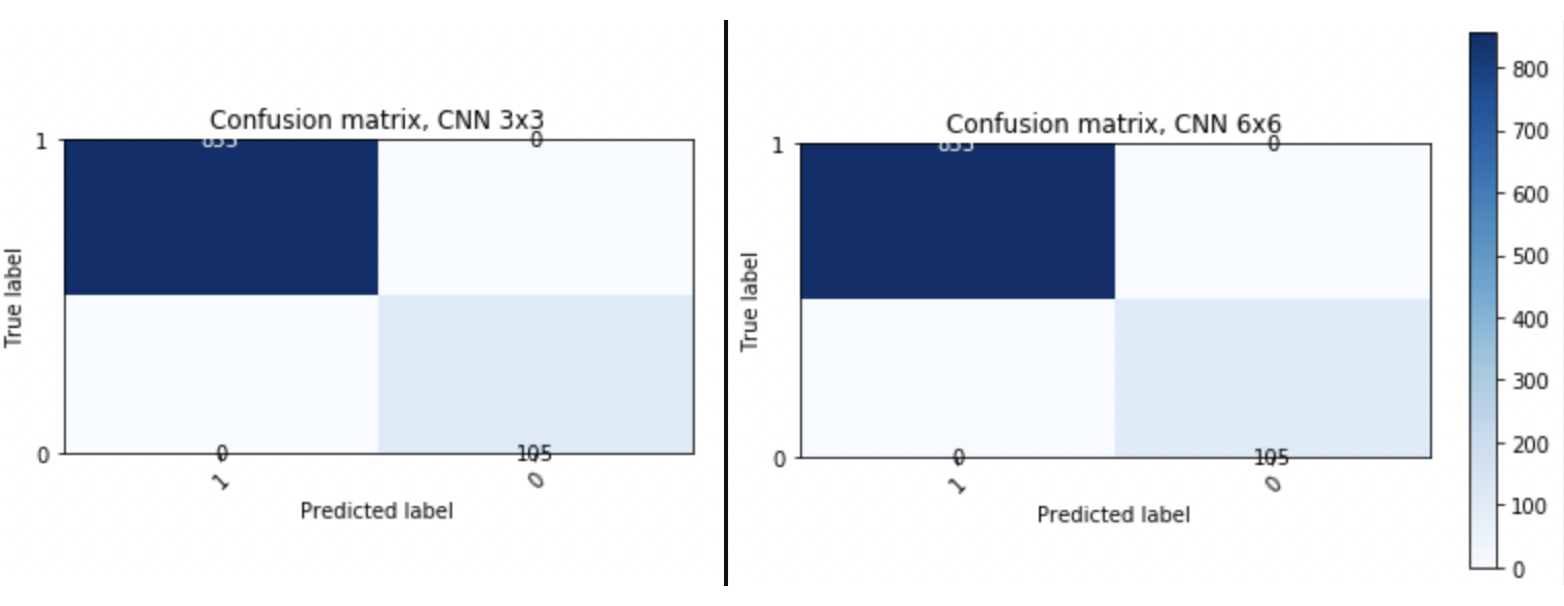
\includegraphics[width=8cm]{confusion_matrix.png}
	\\Fig \ref{confusion_matrix}: This is the confusion matrix from the 3x3 and 6x6 filter training.
	\centering
\end{figure}

%\begin{center}
%	\label{confusion_matrix}
%	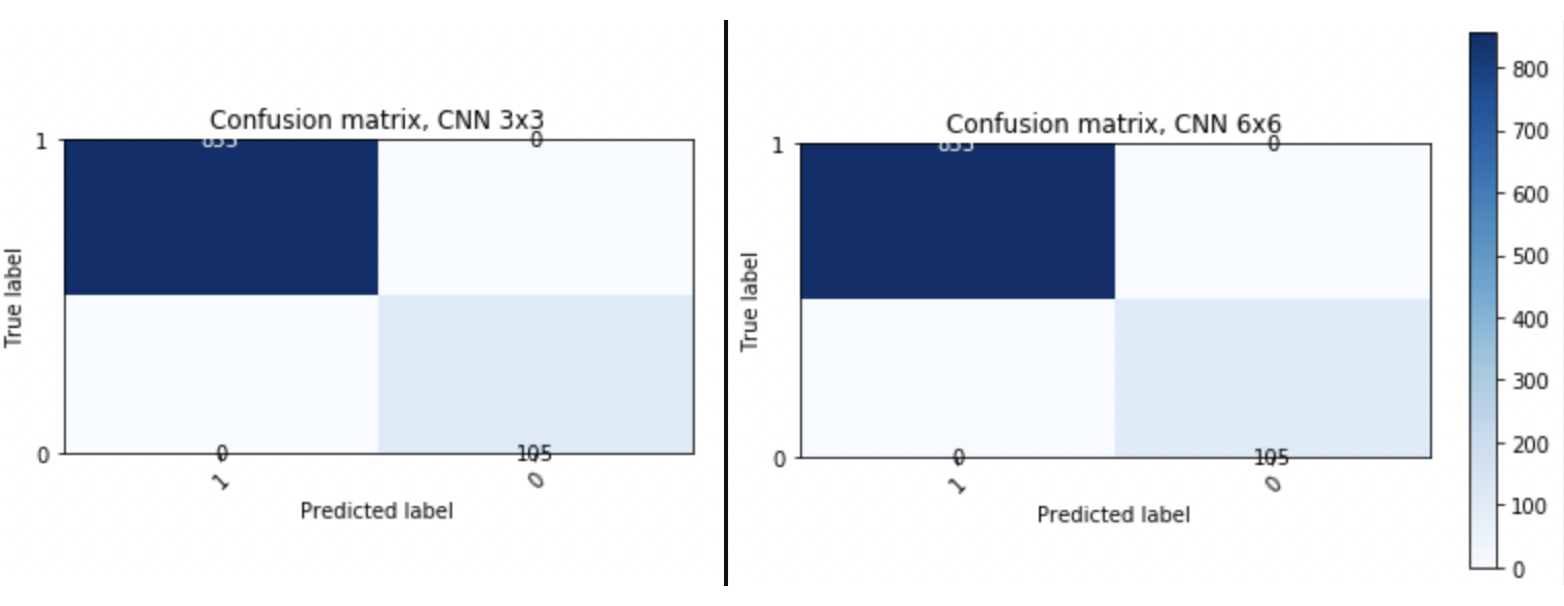
\includegraphics[width=8cm]{confusion_matrix.png}
%\end{center}


\begin{center}
	\begin{tabular}{ |c|p{1.5cm}|p{2.25cm}|p{2.25cm}|p{2.25cm}| } 
		\hline
		 & CCN Taining Time & 2 Step Sliding Window & 5 Step Sliding Window & 10 Step Sliding Window \\
		\hline
		\multirow{3}{4em}{3x3 Filter} & 6.91 sec & 708.19 sec & 716.51 sec & 1060.81 sec \\ 
		
		& 7.11 sec & 860.16 sec & 861.87 sec & 881.87 sec  \\ 
		& 6.50 sec & 637.75 sec & 641.66 sec & 856.81 sec \\ 
		\hline
		\multirow{3}{4em}{6x6 Filter} & 9.85 sec & 1486.03 sec & 767.54 sec & 783.68 sec \\ 
		& 11.65 sec & 1035.58 sec & 909.84 sec & 881.36 sec \\ 
		& 9.35 sec & 757.05 sec & 753.31 sec & 955.60 sec \\ 
		\hline
	\end{tabular}
\end{center}

Both the 3x3 and 6x6 CNN's had 100\% accuracy while training, which fig \ref{confusion_matrix} shows. The results of the CNN with a filter of 3x3 trained quicker than the CNN with a filter of 6x6. These outcomes were the same in all three trials. All the trials found all of the red dots, but the quickest was the 3x3 2 step SW's third trail, with a time of 637.75 seconds while the 6x6 2 step window was the slowest at 1486.03 seconds. All of the 3x3 with a 2 step window was generally the quickest from their runs. However, for the 6x6 filter with a 5 step SW, results were quicker than the other 6x6 results, but still not as fast as the 3x3 2 step SW. On average, we found the 6x6 filter took about 3 seconds longer to train the model.
\section{Discussion}
%note: maybe insteead of finding the highest \% patch, using the predicted label might have worked as well.
%Increasing dense layers node number-> will incrase training time but should make predictions better, therefore potentially speeding upu the overall game.

We can see from the results that the most effective method was to use a 3x3 filter within the CNN and SW that is stepping a step of 2. Even though the SW stepping two steps was the slowest, taking 0.01 seconds while the others took 0.00 seconds, the overall experiments completed the quickest. We believe this is due to the CNN training with higher accuracy results, and with the SW moving only two steps, was able to break the image into more patches allowing more chance of the patches matching up. Therefore, even though the SW took longer, with the more patches to be able to predict with, it meant that the program was less likely to make wrong predictions and having to keep searching around the room. It was, therefore, making the entire process a lot quicker. However, there were occasions, with a 6x6 filter that had either a 5 or 10 step SW, that the program kept going circling, searching for the red dot until it got found. Sometimes after taking more than two full rotations till it found the dot.

The program was able to complete all the required task of collecting all the dots. However, there were some results that we did not initially expect. In regards to the 6x6 filter, we expected that the accuracy of the predictions would be lower than the 3x3. However, we did not expect the overall time to take longer than the 3x3 filter. We acknowledge that more calculations get done in each filter, but by covering more of the overall image, we expected it to be of a similar time or possibly quicker. We believe more exploring into these parameters is needed by the author.

We can see that in every run, for each setting, the program was able to find all eleven dots within the map. However, we feel that there are other ways ta achieve this, which could potentially improve the complexity and run time of the algorithm and speed up the overall process. 

\section{Conclusion}

Overall, the CNN with the 3x3 filter and using a 2 step SW performed the best. In both terms of being the fastest to train and being the quickest to complete collecting all the dots. Therefore, showing that the trade-off of steps and accuracy is not worth pursuing within this case. However, the 6x6 filter worked best with a 5 step SW. We believe that more exploring into the effect the CNN's dense layers and the parameters need to be experimented on, to see if increase the dense layers will see a benefit in the increase filter size and over performance time, compared to the 3x3. Interestingly when the 6x6 filter increased its SW steps, the program finished quicker than when it did with a 2 step SW. 

We believe more research needs carrying out into the trade-off between training time and the step of SW to see if, by increase layers and density of CNN, while would take the training time longer, but would it speed up the overall process. Especially when looking at the bigger filter and the higher SW steps, to see what the correlation between these two factors are.


%\medskip
%\newpage
%\begin{appendices}
%	\section{Total count for Country}
%	\label{appendix:totalcountall}
%	%% Add image of graph here.
%	%\includegraphics[scale=0.5]{totalcount}
%	
%	\section{Lift Table of Items Whole Dataset}
%	\label{appendix:wholelift}
%	%\includegraphics[scale=0.2]{wholelift}

%	\section{Confidence Table of Items Whole Dataset}
%	\label{appendix:wholeconf}
	%\includegraphics[scale=0.2]{wholeconf}
	
%	\section{Lift Table of United Kingdom Items}
%	\label{appendix:uklift}
	%% Add image of graph here.
	%\includegraphics[scale=0.2]{uklift}
	
%	\section{Confidence Table of United Kingdom Items}
%	\label{appendix:ukconf}
	%\includegraphics[scale=0.2]{ukconf}
	
%	\section{Lift Table of Germany Items}
%	\label{appendix:germanylift}
	%\includegraphics[scale=0.2]{germanylift}
	
%	\section{Confidence Table of Germany Items}
%	\label{appendix:germanyconf}
	%\includegraphics[scale=0.2]{germanyconf}
	
%	\section{Lift Table of France Items}
%	\label{appendix:francelift}
	%\includegraphics[scale=0.2]{francelift}
	
%	\section{Confidence Table of France Items}
%	\label{appendix:franceconf}
	%\includegraphics[scale=0.2]{franceconf}
	
%	\section{Lift Table of Erie Items}
%	\label{appendix:eirelift}
	%\includegraphics[scale=0.19]{eirelift}
	
%	\section{Confidence Table of Eire Items}
%	\label{appendix:eireconf}
	%\includegraphics[scale=0.19]{eireconf}
	
%\end{appendices}

%\newpage

%Sets the bibliography style to UNSRT and imports the 
%bibliography file "samples.bib".
\bibliographystyle{acm}

{\footnotesize
	\bibliography{samples}
}


\end{document}